\newpage
\subsubsection*{Component-and-Connector View}

The view displays high-level communication between the subsystems and how they should work as a whole. Connections are defined by various communication channels and their protocols.
\vspace{3mm}

Apart from the usual interaction of the browser, web and back-end application trio, the Docker Swarm component introduces few key interactions. The back-end application plays a key role as it queries resources from the database, while providing metrics via Serilog and DataDog Agent to the DataDog Logging Service. It also communicates with SonarQube - the Static Code Analysis tool in the form of analysis reports.System telemetries are gathered and envisioned with the interaction of Prometheus and Grafana. The metrics pulled from the back-end application by Prometheus are gathered by Grafana using PromQL. It is then displayed on dashboards to analyse those.
\vspace{3mm}

\begin{figure}[h!]
    \centering
    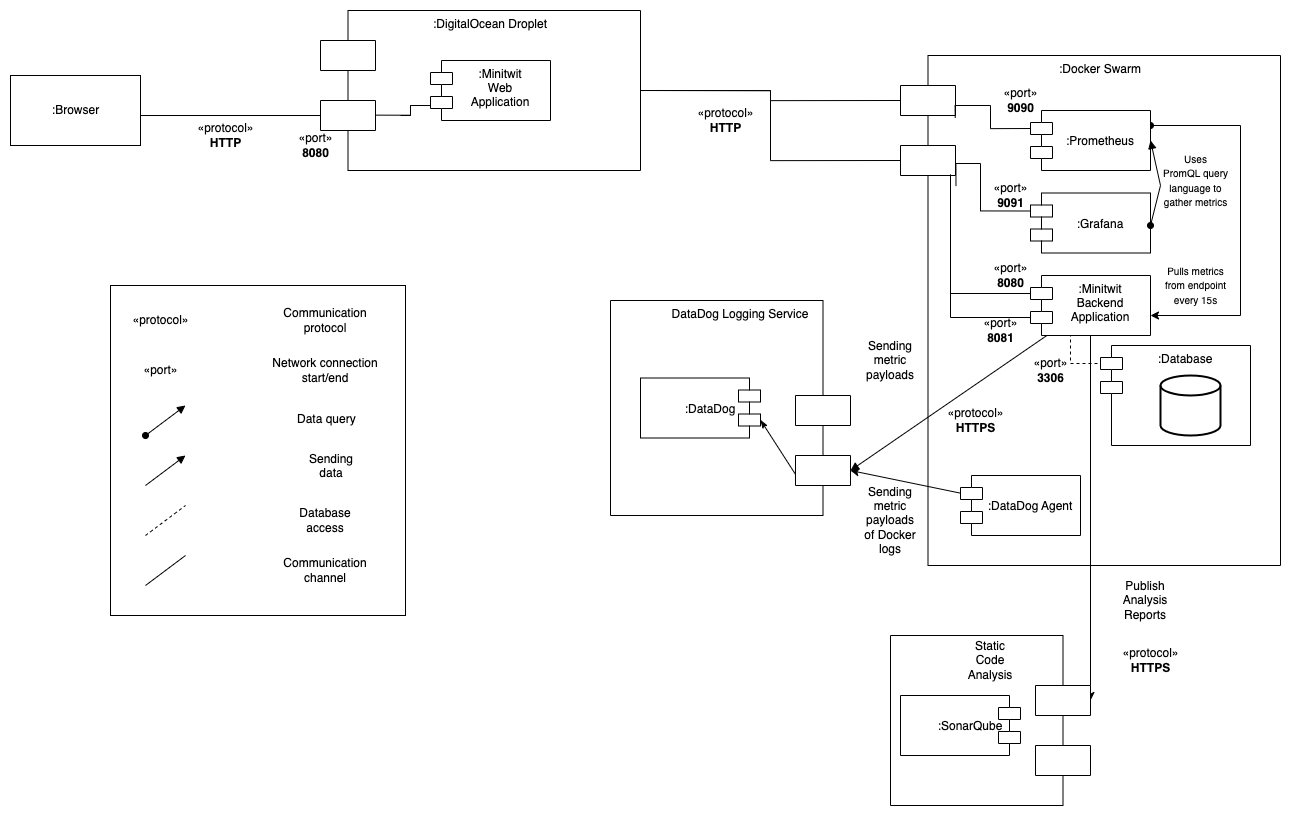
\includegraphics[width=\linewidth,height=\textheight,keepaspectratio]{images/architectural_views/minitwit_cc_view.png}
    \caption{Component-and-Connector View ~\cite{componentAndConnectorView}}
    \label{fig:ccview}
\end{figure}